%; whizzy chapter
% -initex iniptex -latex platex -format platex -bibtex jbibtex -fmt fmt
% 以上 whizzytex を使用する場合の設定。

%     Kansai Debian Meeting resources
%     Copyright (C) 2007 Takaya Yamashita
%     Thank you for Tokyo Debian Meeting resources

%     This program is free software; you can redistribute it and/or modify
%     it under the terms of the GNU General Public License as published by
%     the Free Software Foundation; either version 2 of the License, or
%     (at your option) any later version.

%     This program is distributed in the hope that it will be useful,
%     but WITHOUT ANY WARRANTY; without even the implied warranty of
%     MERCHANTABILITY or FITNESS FOR A PARTICULAR PURPOSE.  See the
%     GNU General Public License for more details.

%     You should have received a copy of the GNU General Public License
%     along with this program; if not, write to the Free Software
%     Foundation, Inc., 51 Franklin St, Fifth Floor, Boston, MA  02110-1301 USA

%  preview (shell-command (concat "evince " (replace-regexp-in-string "tex$" "pdf"(buffer-file-name)) "&"))
% 画像ファイルを処理するためにはebbを利用してboundingboxを作成。
%(shell-command "cd image200708; ebb *.png")

%%ここからヘッダ開始。

\documentclass[mingoth,a4paper]{jsarticle}
\usepackage{kansaimonthlyreport}
\usepackage[dvips]{xy}
\usepackage{ulem}

% 日付を定義する、毎月変わります。
\newcommand{\debmtgyear}{2013}
\newcommand{\debmtgdate}{28}
\newcommand{\debmtgmonth}{4}
\newcommand{\debmtgnumber}{71}

\begin{document}

\begin{titlepage}

% 毎月変更する部分、本文の末尾も修正することをわすれずに

 第\debmtgnumber{}回 関西 Debian 勉強会資料

\vspace{2cm}

\begin{center}
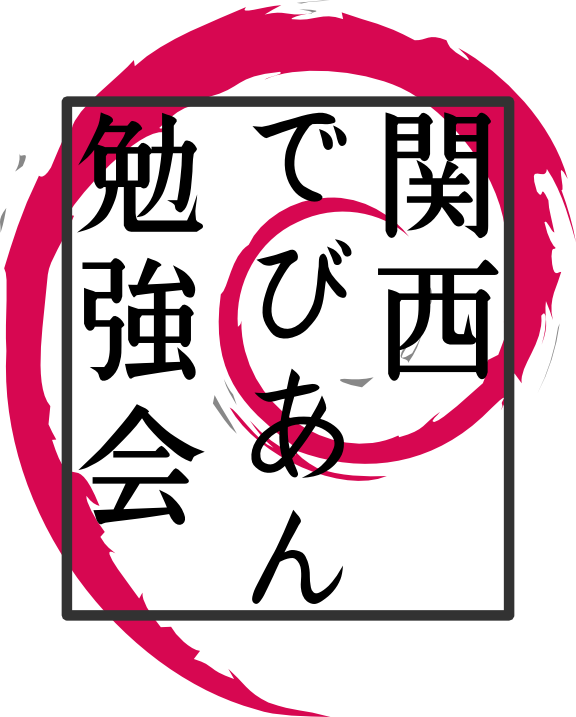
\includegraphics{image200802/kansaidebianlogo.png}
\end{center}

\begin{flushright}
\hfill{}関西 Debian 勉強会担当者 佐々木・倉敷・のがた・かわだ・八津尾 \\
\hfill{}\debmtgyear{}年\debmtgmonth{}月\debmtgdate{}日
\end{flushright}

\thispagestyle{empty}
\end{titlepage}

\dancersection{Introduction}{Debian JP}

\vspace{1em}

 関西Debian勉強会はDebian GNU/Linuxのさまざまなトピック
 (新しいパッケージ、Debian特有の機能の仕組、Debian界隈で起こった出来事、
 などなど)について話し合う会です。

 目的として次の三つを考えています。
 \begin{itemize}
  \item MLや掲示板ではなく、直接顔を合わせる事での情報交換の促進
  \item 定期的に集まれる場所
  \item 資料の作成
 \end{itemize}

 それでは、楽しい一時をお楽しみ下さい。

\newpage

\begin{minipage}[b]{0.2\hsize}
 {\rotatebox{90}{\fontsize{80}{80}
{\gt 関西 Debian 勉強会}}}
\end{minipage}
\begin{minipage}[b]{0.8\hsize}
\hrule
\vspace{2mm}
\hrule
\setcounter{tocdepth}{1}
\tableofcontents
\vspace{2mm}
\hrule
\end{minipage}

\dancersection{最近のDebian関係のイベント報告}{Debian JP}

\subsection{第 70 回関西 Debian 勉強会}

70 回目の関西 Debian 勉強会は 3 月 24 日(日)に港区民センターで行なわれ
ました。

あわしろいくやさんの「UbuntuとGNOME Shellと私」は GNOME Shell の便利な
使い方、拡張機能との付き合い方といった内容でした。

八津尾さんの「管理者視点からのGNOMEの大規模な配置」は Josselin Mouette
さんの「Large deployment of GNOME from the administrator perspective」
プレゼン資料を元に GNOME を読みといてみました。
ざっくりと GNOME の内部構造がとらえられたのではないかと思います。まだ
よくわからないところがありますので後追い企画も考えてみたいところです。

\subsection{第 99 回東京エリア Debian 勉強会 2013 年 4 月 勉強会}
4 月 20 日(土) にあんさんぶる荻窪 第一教室で、東京エリア Debian 勉強会
が開催されました。

杉本さんによる「debootstrapを有効活用してみよう」、たかはしさんによる
「Debianの認証をWindowsに統合してみたり」、山本さんによる「PowerPC の
Vector Facility や Vector-Scalar Floating-Point Operation の Opcode
Map を調べてみた。」の発表が行なわれました。

たかはしさんの発表は昨年、関西でも何度か行なった認証回りのお話しですの
で参考にしてみてください。

\subsection{Debian Project}

Debian Project リーダ選挙が行なわれ、Lucas Nussbaum さんが新しいプロジェ
クトリーダに選出されました。
3 期に渡ってプロジェクトリーダを務められた Stefano Zacchiroli さん、あ
りがとう。

今年の DebConf13 は スイス、ヴォーマルキュの Le Camp で開催されますが、
来年の DebConf14 が、アメリカ、オレゴン州ポートランドで開催されること
が決定しました。
\footnote{\url{http://lists.debian.org/debian-project/2013/04/msg00039.html}}

リリースチームより、5 月 4 日、5 日の週末目標に wheezy をリリースする
と告知がありました。
\footnote{\url{http://lists.debian.org/debian-devel-announce/2013/04/msg00006.html}}
フリーズしてからもうすぐ 1 年というところでようやく wheezy がリリース
されます。みなさんリリースパーティの準備をしましょう。

\dancersection{事前課題}{Debian JP}

今回は以下の課題を出題しました.
\begin{screen}
  \begin{enumerate}
  \item %
    「\href{http://www.debian.org/releases/wheezy/releasenotes}{%
      Debian 7.0 -- リリースノート}」を読んできてください。

    誤植や誤訳などの気づいたこと、わからないなと思うことなどがあれば教え
    てください。

    \url{http://www.debian.org/releases/wheezy/releasenotes}
  \item %
    Debian をこれから使ってみようとされている方は Debian もしくは wheezy
    に対して気になっていることがあれば教えてください。
  \item %
    Debian をすでにお使いの方は squeeze から wheezy へのアップグレードで
    はまりそうなところ、気になるところがあれば教えてください。

    もしくは、お使いの squeeze 環境を一つ、wheezy にアップグレードしてみ
    て下さい。そしてその結果を教えてください。
  \item %
    クラウド的なものをさわったことのない方は、(あれば)理由を教えてくださ
    い。ある人は、セッション中にいろいろツッコミしてください。

  \end{enumerate}
\end{screen}
参加者の皆さんの解答は以下の通りです:

\begin{prework}{ kozo2 }
  \begin{enumerate}
  \item %
    すみません着くまでに読みます
  \item %
    \begin{description}
    \item[Debianに対して] \\
      Firefoxをinstallする方法はppaを追加するしか無いのでしょうか。
    \item[wheezyに対して] \\
      たしかkernelのversionが3.2あたりではなかったでしょうか。
      sidにせずwheezyのままkernelやその他のpackageを新しくすることは可能でしょうか。
      というのはsidではskypeのinstallができなかった記憶があるので。
    \end{description}
  \item %
    いつもsidにしていたので書けません。すみません。
  \item %
    あるのでセッション中に伺います。AWSはすごく興味があるので。研究系の現場でもAWSを使った方がいい状況になっていると思うのですが恐らく日本ではAWSにお金を使わせてもらっているところはまだ(ほとんど)無いのではないかと思うので。
  \end{enumerate}
\end{prework}

\clearpage

\begin{prework}{ 佐々木洋平 }

  \begin{enumerate}
  \item %
    発表に備えて \texttt{git svn clone ...} と叩いたら, なかなか clone 終わらなくて歴史を感じている次第です.
  \item %
    普段から使っておりますので...
  \item %
    リモートでデスクトップの upgrade をしたら, 起動しなくなる事案が発生しました.
    %
  \item %
    VPS として S@@Ses のVPS を複数台使っているぐらいですが, これはクラウドなんでしょうか?
    Xen 環境なのでカーネルを上げられないのがちょっと辛いですが, それ以外はまあなんとか.
    というか,
    そもそもクラウドって何ですか?

    AWS 自体は使ってみたいとは思ってましたが, 以前の状況では予算の都合で諦めました.
    そのうち触ってみようと思います.
  \end{enumerate}
\end{prework}

\begin{prework}{ かわだてつたろう }
  \begin{enumerate}
  \item %
    これから読みます。
    \setcounter{enumi}{2}
  \item %
    Debian 以外のパッケージを使用していると multiarch, /run 周りではまりそうな気がします。
  \item %
    特に理由は無いのですが、さわったことがないです。
  \end{enumerate}
\end{prework}

\begin{prework}{ 山城の国の住人 久保博 }
  \begin{enumerate}
  \item %
    はい、これから読みます。
  \item %
    もう使いましたので…
  \item %
    気になることをいくつか挙げます.
    \def\theenumii{\alph{enumii}}
    \def\labelenumii{\theenumii.~}
    \begin{enumerate}
    \item %
      \texttt{/etc/X11/xorg.conf} が存在したら、アップグレード前に名前を変えて取っておく方が良いと思います。おそらく、そのまま存在すると却って邪魔です。
    \item %
      X の反応が却って悪くなりました。カーネルモードのドライバに移行したからでしょうか。
    \item %
      カーネルまわりで多くのバグレポートが残っているので、古めのハードウェアやちょっと変わったデバイスがあったりするとはまるかも。バグレポートは見ておくといいかもしれません。 私は一つ踏んづけました。
    \item %
      ノートPCで、時々ブート途中にコンソールが消えて画面が真っ暗になるようになりました。dm-crypt のパスワードを入力する所なので、困ってます。
    \item %
      GNOME3 初心者は、dist-upgrade 後に reboot する前に、 gnome-shell-extensions パッケージをインストールすることをお勧めします。
    \item %
      ruby 関係の移行には気をつけたい
    \item %
      dist-upgrade が disk fullで途中で止まっても諦めるな。要らないものを消して、 -f オプションで切り抜けろ。
    \end{enumerate}
  \item %
    クラウド的なものはほとんど使っていません。新しいものに適応する力が弱っているので。
  \end{enumerate}
\end{prework}

\clearpage

\begin{prework}{ 甲斐正三 }
  事前課題にお答えします。
  \begin{enumerate}
  \item %
    kernel upgrade についても触れていただきたい。
  \item %
    特にありません。
  \item %
    Debian Squeeze上のqemu-kvmにDebian Squeezeの
    ベースシステムとデスクトップシステムを新規インストー
    ルし、これをWheezyにアップグレードしてみました。
    気付いた点は以下の3点でした。
    \def\theenumii{\arabic{enumii}}
    \def\labelenumii{(\theenumii)~}
    \begin{enumerate}
    \item %
      upgrade中、パネル上のepiphanyのアイコンが消えて、グレーの四角になる。
    \item %
      「GNOME3の読み込みに失敗しました。」メッセージが出て
      フォールバックする。VM上のwheezy/sidも同様。
    \item %
      kernelが、'3.2.0-2-amd64'にならず、リリースノートに
      その説明もない。'Linux kvm-sqz 2.6.32-5-amd64'のまま。
      'dist-upgrade'したのち、'apt-get install linux-image-3.2.0-2-amd64'で
      インストールした。インストール成功。
    \end{enumerate}
  \item %
    触ったことがありません。
    理由:差し迫った必要性がない。
  \end{enumerate}
\end{prework}

\begin{prework}{ 川江 }
  \begin{enumerate}
  \item %
   細かく見ていませんが、ないような気がします。
 \item %
   compizは使えるようになりました?
 \item %
   もともと、wheezyなのでどうしましょう?
 \item %
   これから「自宅クラウド」を作ろうと思っていすので。
 \end{enumerate}
\end{prework}

\begin{prework}{ 大林 }
  \begin{enumerate}
  \item %
   一通り目を通しました。行くまでにもう少しじっくり読みます。
   \setcounter{enumi}{2}
 \item %
   なにかありますかねえ。以前squeezeへアップグレードしたときには特に問題なくできたのでなんとかなる気がしています。
 \item %
   つかったことはありません。
 \end{enumerate}
\end{prework}

\clearpage

\begin{prework}{ 西山和広 }
  \begin{enumerate}
  \item
    \begin{itemize}
    \item %
      ch-upgrading で sources.list だけではなく sources.list.d への言及もあった方が良いのではないかと思いました。
    \item %
      4.5.8. コンソール接続へセッションの変更:
      \begin{commandline}
        > 異なったテキストモードのターミナル間で切り替えを行うには、Alt+左矢印 か Alt+右矢印 も使えます。
      \end{commandline}
      \noindent
      「異なった」は「ターミナル」にかかると思うのですが、「テキストモード」にかかっているように見えてしまいます。
    \item %
      4.5.9.1. Sudo:
      「visudo -f」はおすすめなので、もっと知られると良さそうです。
    \item %
      4.5.9.2 Screen:
      tmux はどうなのか気になりました。
    \item %
      4.8. 廃止予定のコンポーネント:
      まだないのは後で書かれる予定でしょうか?
    \item %
      4.9. 時代遅れ (Obsolete) のパッケージ:
      \begin{commandline}
        >portmap: 後継となるパッケージは rpcbind です。
      \end{commandline}
      \noindent
      /etc/hosts.allow などで tcp wrapper の設定をしている場合は変更が必要なのかどうかが気になりました。
    \item %
      5.2. LDAP サポート:
      「 libnss-ldap パッケージを、すべての LDAP 検索に分割されたデーモン (nslcd) を使っている新しいライブラリである libnss-ldapd に置き換えることをお勧めします。libpam-ldap の代替品は libpam-ldapd です。 」
      のところがわかりにくい気がしました。
    \item %
      5.9. pdksh から mksh への移行:
      PS1 が pre になっているのは意図的なのでしょうか? (原文でも同じ)
    \item %
      6.2. 助けを求めるには:
      日本語訳には訳注で debian.or.jp の情報を付け足しても良いのではないかと思いました。
    \item %
      A.3. 古く不要になった設定ファイルを削除する:
      「*.dpkg-\{new,old\}」の他に「smb.conf.ucf-dist」のような「*.ucf-*」も書いてあった方が良いのではないかと思いました。
    \end{itemize}
    \setcounter{enumi}{2}
  \item %
    Ubuntu 10.04 から Ubuntu 12.04 で nslcd の変更により 1 文字のユーザー名や smbldap-tools で設定された空白の入ったグループ名 (Domain Users など) が見えなくなっていて、 /etc/nslcd.conf で
    \begin{commandline}
# allow name with only 1 char and spaces (e.g. "Domain Users")
validnames /^[a-z0-9.\_{}@$]([ a-z0-9.\_{}@$\\~-]*[a-z0-9.\_{}@$~-])?$/i
    \end{commandline}
    \noindent
    という設定を入れたので、 squeeze から wheezy へのアップグレードでも同じ問題にはまりそうだと思いました。
  \end{enumerate}
\end{prework}

\begin{prework}{ おくの }
  \begin{enumerate}
  \item %
    読みました。リリースが楽しみです。
  \item %
    Multiarchが気になります。
  \item %
    新規インストールするつもりなので……
  \item %
    四月からクラウドをやるかもしれない会社に転職したので、勉強中ですです。
  \end{enumerate}
\end{prework}

\clearpage

\begin{prework}{ lurdan }
  \begin{enumerate}
  \item %
   ざっくり読みましたが、特に気になる点はありませんでした。一部未訳部分がありますが、更新中なので仕方ありませんね。
 \item %
   もう使ってます。
 \item %
   特に気になることはありません。
 \item %
   ツッコミお待ちしております
 \end{enumerate}
\end{prework}

\clearpage
\dancersection{%
  リリースノートを読んでみよう}{%
  佐々木洋平}

\subsection{はじめに}

04/18 に \texttt{debian-devel-announce} ML に
「FINAL release update」という件名のメールが流れました
\footnote{\url{http://lists.debian.org/debian-devel-announce/2013/04/msg00006.html}}.
このメールの冒頭に
\begin{commandline}
Timings
=======

We now have a target date of the weekend of 4th/5th May for the release.
We have checked with core teams, and this seems to be acceptable for
everyone. This means we are able to begin the final preparations for a
release of Debian 7.0 - ``Wheezy''.

The intention is only to lift the date if something really critical pops
up that is not possible to handle as an errata, or if we end up
technically unable to release that weekend (e.g. a required machine
crashes or d-i explodes in a giant ball of fire). Every other RC fix
that does not make it in time will be r1 material. Please be sure to
contact us about the RC fixes you would like included in the point
release!
\end{commandline}
\noindent
とある通り, Wheezy のリリースは 05/04 or 05/05 が予定されています.

そんなわけで, 本発表の趣旨は
「現状のリリースノートを読んで wheezy の状況を把握しよう!」です.
%
個人的な観測では, 関西Debian勉強会参加者の多くが
普段使いの環境は \texttt{unstable} or \texttt{stable} なので,
現状の \texttt{testing}, すなわち wheezy を使っていない気がします.
%
freeze 期間なので \texttt{unstable} と \texttt{testing} の違いは
微々たるモノかもしれません.
%
ですが, それなりに違いがあるハズです
\footnote{%
  %
  来月にリリースがなされる訳で, その後に「Debian を使ってみよう!(キリッ)」
  と他人に勧める際にも, 勧める我々(私?)が
  %
  「いや〜ふだん\texttt{stable}使ってないから良くわからんわ〜」では,
  %
  ちょっとアレですよね, という気持ちもあります.
}

それでは
\begin{commandline}
  原版:
  http://www.debian.org/releases/wheezy/amd64/release-notes/index.html

  日本語訳:
  http://www.debian.org/releases/wheezy/amd64/release-notes/index.ja.html
\end{commandline}
\noindent
を開いて, 読んで行きましょう.
余裕のある人は
\begin{commandline}
  $ svn co svn://svn.debian.org/ddp/manuals/trunk/release-notes
\end{commandline}
% $
\noindent
として, 原文を修正しつつ進めるのが良いかもしれません.

\clearpage
\dancersection{%
クラウド初心者が AWS に Debian をのっけて翻訳サービスの試行に挑戦してみた}{%
倉敷 悟
}

基本的にクラウドを使うことにあまり興味がない (作ることには興味あるけど) という
こともあって、これまでいわゆるクラウドというものと無縁に生きてきました。今回、
たまたま使ってみる用事ができたこともあって、クラウド上で Debian を動かしてみま
したので、顛末をご紹介します。

\subsection{AWS に目が向いた背景}

私は自宅以外のコンピュータ資源として、さくらの(共用)レンタルサーバと、実家に
置いた安売りサーバ、いわゆる自宅サーバを使用しています。主な用途は、携帯
キャリア/プロバイダの都合から影響を受けないように独自ドメインの転送メール
アドレスを保持すること、及び自分用にサーバサービスを提供すること、あとはちょっと
した実験、といったところです。

さくらのレンタルサーバは、古式ゆかしき /home 切り売り CGI 環境しかないので、今と
なっては動かせるアプリケーションが極端に限定されます。また、実家サーバは回線が
ADSL で帯域もなく、時折不安定に IP がつけかわったりするので、自分以外の誰かに
アクセスさせるには向いていません。
ですが、Debian JP の翻訳の絡みで、ちょっとだけ「不特定多数からアクセスされ(得)る」
環境が欲しくなりました。一応実験のための一時的な設置と考えてはいますが、数ヶ月
くらいは動かすことになるだろうし、IP も固定である方がよく、動かす対象は Python の
django で書かれたプロセス常駐型の Web DB アプリケーションです。

そこで、VPS としても使えるらしいのと、周囲で推しの声が多数観測されていたこともあり、
AWS の「初期利用1年無料枠」を使ってみることにしました。使えるリソースは AWS 的に
最小限ですが、機能の試用や検証を 1 年かけてできるということなので、結構な大盤
振る舞いだと思います。ありがてぇありがてぇ。

\subsection{簡単な事前調査}

\subsubsection{AWS の概略}
AWS と一口に言っても、中身はそれぞれ異なるサービスの総称です。ざっくり数えてみた
ところ、25 個ほどありました。そのうち 10 個くらいのサービス名は略語で、一見した
ところではさっぱり意味がわかりません。
AWS では Elastic という用語がよく使われているようですので、E は Elastic、A は Amazon、
S は Service、程度のあたりはつきますが、最初は謎の略語名に圧倒されてしまうかも
知れません。今回試してみた EC2 だと、Elastic Computing Cloud の省略です。ECC だと
いろいろヤバかったのかも知れませんね。

ちなみに Elastic の意味は「伸縮自在」といったところです。

\subsubsection{AWS の特徴}
AWS は、いわゆるレンタルサーバや VPS とは違って、リソースが文字通り Elastic です。
画面をポチポチやれば、メモリや CPU パワーなどを自由に変更することができますし、その
変更幅もかなり大きくとれます。また、料金体系も従量課金となっていて、物理的なマシンや
ノードの単位に縛られず、「電気・水道のようにコンピュータ資源を使う」感覚を実現している
といえるでしょう。周辺サービスについても、種類と内容がともに充実しているだけでなく、
日々強化されていっているので、便利さでは他の業者の追従を許していません。いろいろな API
を提供していて、「AWS としての機能」を別のアプリなどから操作できる (らしい) というのも
興味深いところです。
まともに使うと料金は割高なようですが、札束さえつっこめば、インフラの構成に制約されること
なく、小さくはじめたサービスをそのまま拡大していけます。そのため、コンシューマ相手にノるか
ソるかのサービスを提供したい場合や、大規模な設備投資が長期的に見合わない場合などに、
とても良くマッチします。

\subsubsection{Debian の使用}
AWS は、Xen をベースに、RedHat を Amazon 内で魔改造したもので構成されています。残念ながら
Debian の出る幕はないわけですが、その上で動かす AMI と呼ばれる仮想 OS イメージについては、
某荒木さんが Debian のイメージをメンテされていると聞いたことがあったので、今回はそれを使う
ことにしました。

\subsection{やってみた}
\subsubsection{アカウントの準備}
まずは、AWS 上にアカウントを作成する必要があります。途中で必要になるので、クレジットカードと、
着信が受けられる電話を手元に用意しておくといいでしょう。アカウントIDは、物販用の amazon.com
(amazon.co.jp ではない) の情報を流用できます。特に待たされたりすることもありませんし、すぐ完了
できるかと思います。

\subsubsection{EC2 でハマってみる}
AWS には綺羅星のごとくベンリ系のサービスがこれでもか!と並んでいるのですが、
今回は VPS がわりに使うだけですので、とりあえず EC2 で OS インスタンスをたてる
ことにします。

AWS は世界各地にデータセンターをもっており、使用するデータセンターを「リージョン」
として選択できます。日本人が日本人向けのインスタンスをたてるわけなので、
ここでは無難に tokyo リージョンを選びました。また、リージョン内にも「エリア」
として複数のネットワークが存在し、冗長化などに役立てることができるらしいのですが、
今回は単体ホストしか使いませんので、「どこでもええわい」としておきます。

EC2 で使う AMI は公式には Debian のイメージが存在しないので、コミュニティ版を
使うことになります。私はこの部分でなかなか手間取りました。ポイントは、

\begin{itemize}
\item 基本的に用意されている Debian のバージョンは stable
\item 展開した後のログインでは、AMI イメージ毎に特定のログイン名を使う (AWS コンソールで作成した SSH 鍵が起動時にそのユーザにセットされる)
\end{itemize}

あたりでしょうか。私は Wheezy を使うつもりだったので、最初は Wheezy のイメージ名を
検索して使用してみたのですが、なんとログインできません。通常は AMI の情報と
してログインユーザ名が提示されているらしいのですが、見つけられなかったため
諦めました。
幸い、http://wiki.debian.org/Cloud/AmazonEC2Image に情報がまとまっていたので、
ログイン名のわかる Squeeze イメージではじめて、後から dist-upgrade することに
します。余談ですが、dist-upgrade すると grub の処理でコケます。最初から grub
は消しときゃいいのになぁ、とは思いました。

インスタンスが起動したら、固定 IP を割り当てます。AWS コンソールから Elastic IPs
の画面を開き、新しい IP をアサインして、起動したインスタンスとの紐づけを行います。
なんでも Elastic IP はインスタンスで使っている限りは無料らしいのですが、
インスタンスを停止した状態で握り続けていると有料になるそうです。実験などで
一時的に使うだけ、という場合は解放するのをお忘れなく。

EC2 で起動したインスタンスは、デフォルトでは外部からアクセスできないように
ファイアウォールが設定されています。「セキュリティグループ」という画面で簡単に
設定できるので、自分用の ssh と、公開する http のポートを開けるようにします。

これで、ほぼ VPS 気分で使えるサーバができました。ssh でログインすれば、後は
いつも通りの作業をするばかりです。

\subsection{RDS でハマってみる}

AWS にはいくつか DB サービスが用意されていますが、その中でも RDS は、普通の
mysql サーバ (だけじゃないけど) を簡単に利用できるものです。今回は Web DB
アプリケーションを動かすので、せっかくなのでこれも使ってみることにしました。

……といっても、実のところ動かすだけなら特にハマりどころもなく、AWコンソール
でちょこっとパラメータを指定すれば、さくっと mysql があがってきます。
EC2 と同様、セキュリティグループによる通信許可をしてあげる必要はありますが、
拍子抜けするくらい簡単に動きました。しかも、自動でバックアップもとってくれる
ようです。

今回の用途であれば、EC2 インスタンスの中に手動で mysql をセットアップしても
良かったのかもしれませんが、実際に本番で使うなら、これも非常に便利な機能だと
思います。

\subsection{まとめ}

動かしたアプリケーションについてもちょっと紹介しようと思っていたのですが、
残念ながら原稿が間にあわなかったので、そちらは時間があればセッション中に
触れることにします。

最後に、VPS 的に使ってみた所感をまとめておきます。総合すると、自宅サーバの
置きかえにはアリかなー、でも一時的な実験とかでなく、常設するなら VPS の方が
安くつくかなー、といったところです。皆さんが試してみたりする時の参考に
なれば幸いです。

\begin{description}
\item いいところ(無料期間の視点)
  \begin{itemize}
  \item 固定IPを使える
  \item Web サービスを公開して試してもらうのに便利
  \item RDB(mysql)を簡単にセットアップできる
  \item 実験が終わってインスタンスを止めれば、費用は不要
  \item 便利ツールとの連携が楽しそう
  \item 足まわりの運用はすべて忘れてしまえる(バックアップ、HA、セキュリティアップデート、……)
  \end{itemize}
\item 微妙なところ
  \begin{itemize}
  \item 無料期間が終わると、ちょいとお高い (t1.micro 1700円/月、RDS 6000〜/月くらいらしい)
  \item パワフルに使うなら、月額固定の VPS の方がいいかも
  \item サービス多すぎ、変化しまくり、使いこなすのは大変そう \#おっさん
  \end{itemize}
\end{description}

% ページ調整用
% \dancersection{月刊 Debian Policy 「オペレーティングシステム」その2}{担当:のがた}
% すみません。今回もお休みです。
% \clearpage

\dancersection{今後の予定}{Debian JP}

\subsection{関西 Debian 勉強会}

次回、第 72 回関西 Debian 勉強会は 5 月 26 日(日)に福島区民センターで行な
います。
セッション内容は未定ですが、新年度入門ネタ、
\underline{恐らく必ず}リリースされているであろう
Wheezy インストール大会になるんじゃないかと思われます。
月刊 Debian Policy も 9 章後半から再開の予定です。

\subsection{東京エリア Debian 勉強会}

100 回を迎える、第 100 回東京エリア Debian 勉強会は内容未定ですが、荻窪
地域区民センターで 5 月 18 日(土)に開催される予定です。

\subsection{大統一 Debian 勉強会}
今年も、大統一 Debian 勉強会が、6 月 29 日(土)東京の日本大学駿河台キャン
パスで開催されます。
%
Call For Presentation の締切は今日です!!
ネタがあるのにまだ申し込んでいない人は、是非今申し込みましょう。
%
最新情報は公式サイト\footnote{\url{http://gum.debian.or.jp/}}
をご覧ください。
%
また、6 月 29 日の予定を空けて東京行きのチケットを確保しましょう!!


% 冊子にするために、4の倍数にする必要がある。
% そのための調整
\dancersection{メモ}{}
 \mbox{}\newpage
%% \mbox{}\newpage
%% \mbox{}\newpage

\printindex
%\cleartooddpage

 \begin{minipage}[b]{0.2\hsize}
  \rotatebox{90}{\fontsize{80}{80} {\gt 関西 Debian 勉強会} }
 \end{minipage}
 \begin{minipage}[b]{0.8\hsize}

 \vspace*{15cm}
 \rule{\hsize}{1mm}
 \vspace{2mm}
 
\includegraphics[width=2cm]{image200502/openlogo-nd.eps}
 \noindent \Large \bf Debian 勉強会資料\\ \\
 \noindent \normalfont \debmtgyear{}年\debmtgmonth{}月\debmtgdate{}日 \hspace{5mm}  初版第1刷発行\\
 \noindent \normalfont 関西 Debian 勉強会 (編集・印刷・発行)\\
 \rule{\hsize}{1mm}
 \end{minipage}

\end{document}
